\section{}
\label{sec:problem4}
%%%%%%%%%%%%%%%%%%%%%%%%%%%%%%%%%%%%%%%%%%%%%%%%%%%%%%%%%%%%%%%%%%%%%%

On the biological cell data we want to model a repulsive event RF with a Single-site McMC simulation of a Strauss Event RF. This model is specified on conditional form, given the event count $k_D = k$, realizations can be found by
%
\begin{equation}
    \begin{array}{rcl}
        \left[\mathbb{X}_\textrm{D}^S \given k_\textrm{D} = k\right] & \sim & p(\vect{x}_1,\vect{x}_2,...,\vect{x}_k \given k_\textrm{D} = k) \\
         & = & \mathrm{const} \times \prod\limits_{i,j\in \{1,2,...k\}} exp\{-\phi(\vect{x}_i-\vect{x}_j)\}
    \end{array}.
    \label{eq:straureal}
\end{equation}
%
Then let the distance be $\tau_{ij} = |\vect{\tau}_{ij}| \in \reals_\oplus; \vect{\tau}_{ij} = \vect{x}_i - \vect{x}_j$, where $\phi(\tau)$ is given by equation 
\begin{equation}
    \phi(\tau) = \begin{cases}
                    \phi_0; & 0 \leq \tau \leq \tau_0\\
                    \phi_0 exp\{-\phi_1[\tau-\tau_0]\}; & \tau > \tau_0
                \end{cases},
    \label{eq:interfunction}
\end{equation}
where $\tau_0 \in R_\oplus$ and $\phi_0,\phi_1 \in R_+$. This gives the model parameters for the Strauss-model $\vect{\theta} _{pS\given k} = [\tau_0,\phi_0,\phi_1]$. The minimum distance between the points in the cells data, $\tau_0$, is calculated by $\tau_0 = \min\limits_{\{i,j\in k;i\neq j\}} |\vect{x}_i-\vect{x}_j|$. The other parameters is chosen to fit the quantiles of L-interaction function of the realizations from the Strauss Event RF to the L-interaction function of the cells data. An initial guess on the model parameter is done, then compared and changed until a fit is made. This yielding the parameters  $\phi_0 = 7$ and $\phi_1 = 90$ and the minimum distance was calculated to be $\tau_0 = 0.0836$. From this knowledge realizations can be generated, and one is displayed in Figure \ref{fig:repulsive_event_rf}. The comparison between the L-interaction functions of the quantiles of the cell data and the realizations from the Strauss Event RF is shown in Figure \ref{fig:strauss_quant1} and  Figure \ref{fig:strauss_quant2}. 
\begin{figure}
    \centering
    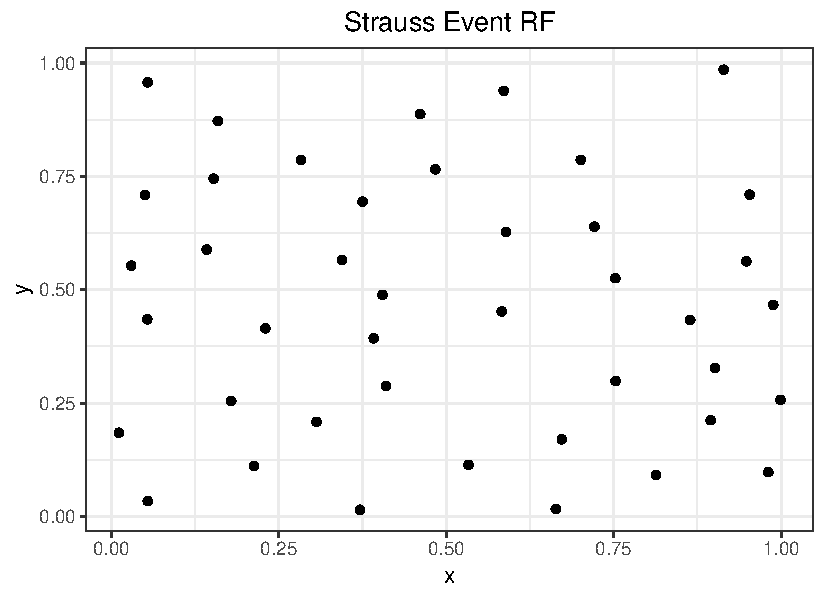
\includegraphics[scale=0.95]{figures/repulsive_event_rf.pdf}
    \caption{One realization of a Single-site McMC simulation of a Strauss Event RF with model parameters $[\tau_0,\phi_0,\phi_1] = [0.84,7,90]$.}
    \label{fig:repulsive_event_rf}
\end{figure}

\begin{figure}
    \centering
    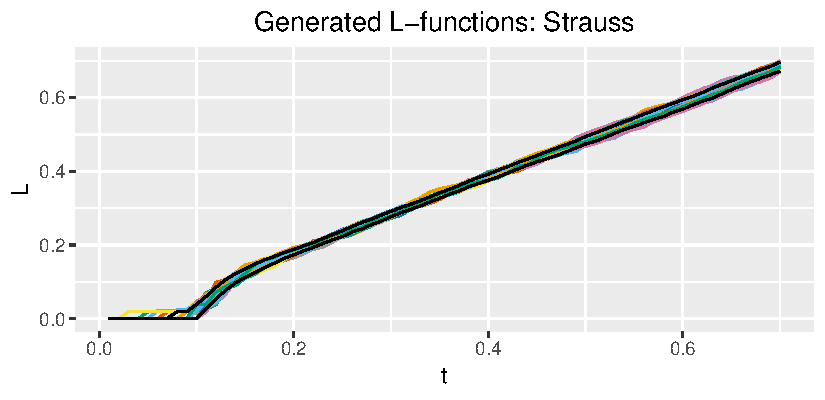
\includegraphics[scale=0.65]{figures/gen_strauss_l.pdf}
    \caption{L-interaction function of $100$ realizations of a Single-site McMC simulation of a Strauss Event RF with model parameters $[\tau_0,\phi_0,\phi_1] = [0.84,7,90]$. The black lines is the $0.05$ and $0.95$ quantile of the L-interaction function.}
    \label{fig:gen_strauss_l}
\end{figure}

\begin{figure}
    \centering
    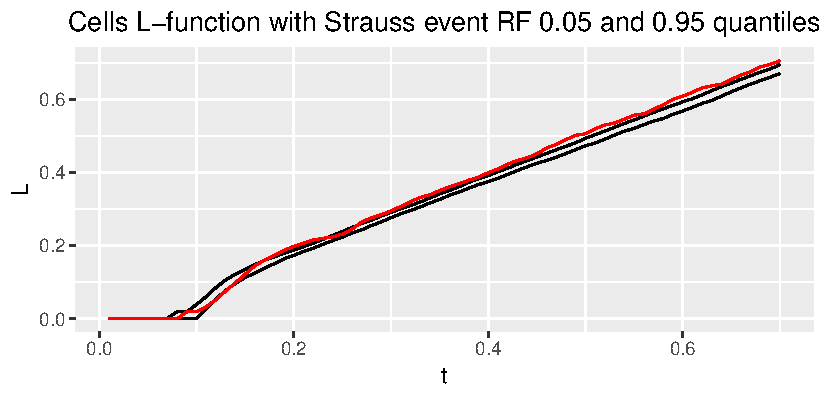
\includegraphics[scale=0.65]{figures/strauss_quant1.pdf}
    \caption{A comparison between the $0.05$ and $0.95$ quantiles of the L-interaction function from $100$ realizations of a single-site McMC simulation of a Strauss Event RF with model parameters $[\tau_0,\phi_0,\phi_1] = [0.84,7,90]$, and the L-interaction function of the biological cell data.}
    \label{fig:strauss_quant1}
\end{figure}

\begin{figure}
    \centering
    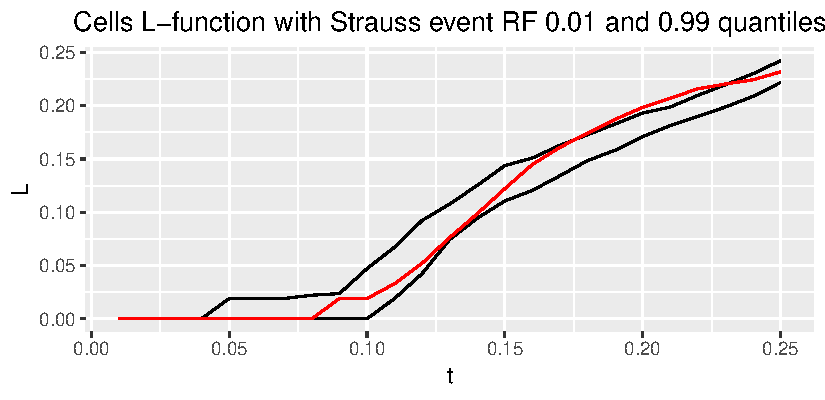
\includegraphics[scale=0.65]{figures/strauss_quant2.pdf}
    \caption{A comparison between the $0.01$ and $0.99$ quantiles of the L-interaction function from $100$ realizations of a single-site McMC simulation of a Strauss Event RF with model parameters $[\tau_0,\phi_0,\phi_1] = [0.84,7,90]$, and the L-interaction function of the biological cell data.}
    \label{fig:strauss_quant2}
\end{figure}

In Figure \ref{fig:strauss_quant1} the L-function of the cells data follows the quantiles for the L-function of the Strauss realizations. From around $t>0.3$ they tend to diverge alittle from eachother, where the L-function for the cells data is a little higher. In the start at from $t=0$ to $t\approx 0.08$, which is around the value of $\tau_0$ the quantiles is $0$ this is, because we have a semi-hardcore model, where we restrict the minimum distance between the points in the realizations. Overall the Strauss model we implemented seems to fit the cells data good, there can still be improvements by choosing better model parameters, but it seems good enough. 